\chapter{Methodology}

\section{Overview}
This chapter outlines the methodology employed for image processing and evaluating the quality of the lens. The process involves several steps, from capturing and preprocessing images to analyzing various lens properties. The chapter also describes the architecture of the system, data flow among the system and features a set of scenarios for simple lens evaluation. This chapter concludes with the design of User Interface Design.

\section{Unconventional Testing Environment}
While professional lens testing typically requires expensive equipment and controlled lighting, this methodology embraces a more accessible "garage lab" approach. Basic household items are repurposed for testing - a white wall becomes the vignetting test surface, while Christmas lights or phone flashlights serve as point light sources for bokeh analysis. This approach, while less precise than industrial solutions, provides meaningful relative measurements that help photographers evaluate their lenses.

\subsection{Calibration Elements}
\subsubsection{DIY Test Charts}
Rather than requiring expensive calibration targets, the methodology relies on printable test charts that users can create at home. A simple grid printed on an office printer serves as a distortion target, while a Siemens star pattern tests resolution. The key is consistency in printing and mounting - charts should be flat and well-lit, even if the absolute precision is lower than commercial targets.

\subsection{Testing Scenarios}

\subsubsection{The White Wall Technique}
The vignetting analysis relies on photographing a uniformly lit white wall. While professional testing uses integrating spheres, a well-lit white wall provides sufficient data for relative comparisons. Users are instructed to position the camera square to the wall and ensure even illumination through test shots.

\subsubsection{Bokeh Analysis Setup} 
Point light sources for bokeh testing can be created using simple LED lights or phone flashlights in a darkened room. The methodology emphasizes consistent testing distances and background separation rather than absolute measurements. This allows meaningful comparisons between lenses even in improvised setups.

\subsection{Environmental Considerations}

\subsubsection{Lighting Compensation}
Rather than requiring expensive studio lighting, the methodology adapts to available light sources. Test procedures include steps for compensating for uneven ambient lighting through reference shots and software correction. This makes testing possible in various environments while maintaining relative accuracy.

\subsubsection{Vibration Management}
Without access to professional vibration isolation tables, the methodology provides techniques for minimizing camera shake using household items. This includes using stacked books as an impromptu stable platform and employing mirror lockup and timer delays to reduce vibration.

\subsection{Consistency Through Process}
While individual measurements may have higher variability than lab tests, the methodology emphasizes consistency through careful documentation and repeated measurements. By averaging multiple tests and following structured procedures, hobbyist photographers can build meaningful datasets about their lens performance using accessible tools and spaces.

\section{Image Acquisition}
\subsection{Camera Control System}
The image acquisition system uses gphoto2 for camera control with:
\begin{itemize}
    \item Automated camera detection and configuration
    \item Exposure and focus parameter management
    \item Error handling and recovery procedures
    \item RAW format capture optimization
\end{itemize}

\subsection{Camera Setup and Configuration}
The image acquisition system employs the gphoto2 library for direct camera control. The system implements a structured approach to camera management with the following key components:

\textbf{Setting Validation}
\begin{itemize}
    \item Parameter range checking
    \item Configuration compatibility verification
    \item Setting application confirmation
    \item Error state recovery
\end{itemize}

\subsection{RAW Image Capture}
The image acquisition process follows a defined protocol:

\textbf{Pre-capture Steps}
\begin{enumerate}
    \item Camera readiness verification with timeout handling
    \item Configuration parameter validation
    \item Memory buffer allocation
    \item Capture target confirmation
\end{enumerate}

\textbf{Capture Process}
\begin{enumerate}
    \item Mirror lock-up if required
    \item Capture command execution
    \item File transfer initiation
    \item Data integrity verification
    \item Local storage management
\end{enumerate}

\subsection{Batch Capture Implementation}
For scenarios requiring multiple captures at different settings:

\textbf{Batch Process Control}
\begin{itemize}
    \item Parameter sequence definition
    \item Automatic setting adjustment between captures
    \item Progress monitoring and status reporting
    \item Error handling with batch continuation capability
\end{itemize}

\textbf{Data Management}
\begin{itemize}
    \item Structured file naming convention
    \item Metadata embedding
    \item Temporary storage management
    \item Dataset organization
\end{itemize}

\subsection{Focus Control System}
The system implements both automatic and manual focus control:

\textbf{Focus Mechanisms}
\begin{itemize}
    \item Autofocus engagement/disengagement
    \item Manual focus drive control
    \item Focus confirmation
    \item Focus distance tracking
\end{itemize}

\subsection{Error Handling and Recovery}
Robust error handling is implemented at multiple levels:

\textbf{Error Categories}
\begin{itemize}
    \item Connection failures
    \item Configuration errors
    \item Capture failures
    \item File transfer issues
\end{itemize}

\textbf{Recovery Mechanisms}
\begin{itemize}
    \item Automatic reconnection attempts
    \item Configuration reset capabilities
    \item Capture retry logic
    \item Resource cleanup procedures
\end{itemize}

\section{Software Architecture Decisions}

\subsection{Dataset Management Architecture}
[To be completed - core data structures, file organization, metadata handling]

\subsection{Camera Control Architecture}
[To be completed - state machine, error handling, event system]

\subsection{Analysis Results Architecture}
[To be completed - result storage, comparison mechanisms, data export]

\section{Image Processing Pipeline}

\subsection{Preprocessing}
Image filtering is a crucial step in image preprocessing; its goal is to enhance the image quality and prepare it for subsequent analysis. Filtering helps in reducing noise, smoothing the image, and highlighting important features.

\textbf{Gaussian blur} is a widely-used smoothing technique that applies a Gaussian function to the image. It effectively reduces noise and detail, providing a smoother and more uniform image. The Gaussian blur is particularly useful in preparing images for feature detection and other analytical processes \cite{gaussian}.

\subsection{Feature Detection}
Feature detection on the captured image is performed using the \textbf{Scale-Invariant Feature Transform} (SIFT). This algorithm detects and describes local features in images, also referred to as keypoints in the following sections. SIFT is used in computer vision for object recognition, image stitching, and other applications due to its robustness to changes in scale, rotation, and illumination. In this case it is used for analyzing sharpness, PSF, and bokeh \cite{Sift}.

\subsection{Analysis Algorithms}
[To be completed - details of each analysis type]

\section{Testing Methodology}

\subsection{Validation Methods}
[To be completed - how results are validated]

\subsection{Comparison Methodology}
[To be completed - comparison with professional tools]

\subsection{Error Analysis}
[To be completed - understanding and quantifying errors]

\section{System Architecture}

\subsection{Component Overview}
The system architecture of the lens evaluation application is composed of four main components: image acquisition, segmentation and preprocessing, lens property evaluation, and result display. These components work together to capture images from a camera, process and analyze these images, and present the results to the user through a web interface.

\subsection{Data Flow}
The data flow in the application follows a structured process from image acquisition to result display. Each step is designed to ensure that the captured images are accurately processed and analyzed, and the results are presented in a user-friendly manner.

\subsection{Integration Points}
[To be completed - how components interact]

\section{User Interface Design}

\subsection{Design Philosophy}
[To be completed - UI/UX principles followed]

\subsection{Interface Components}
The user interface is structured around a main screen for overall navigation and specific screens for various tasks. The main screen serves as the central hub for the application, providing options to load and save datasets, inspect the camera status, and run analyses.

\begin{figure}[h]
\centering
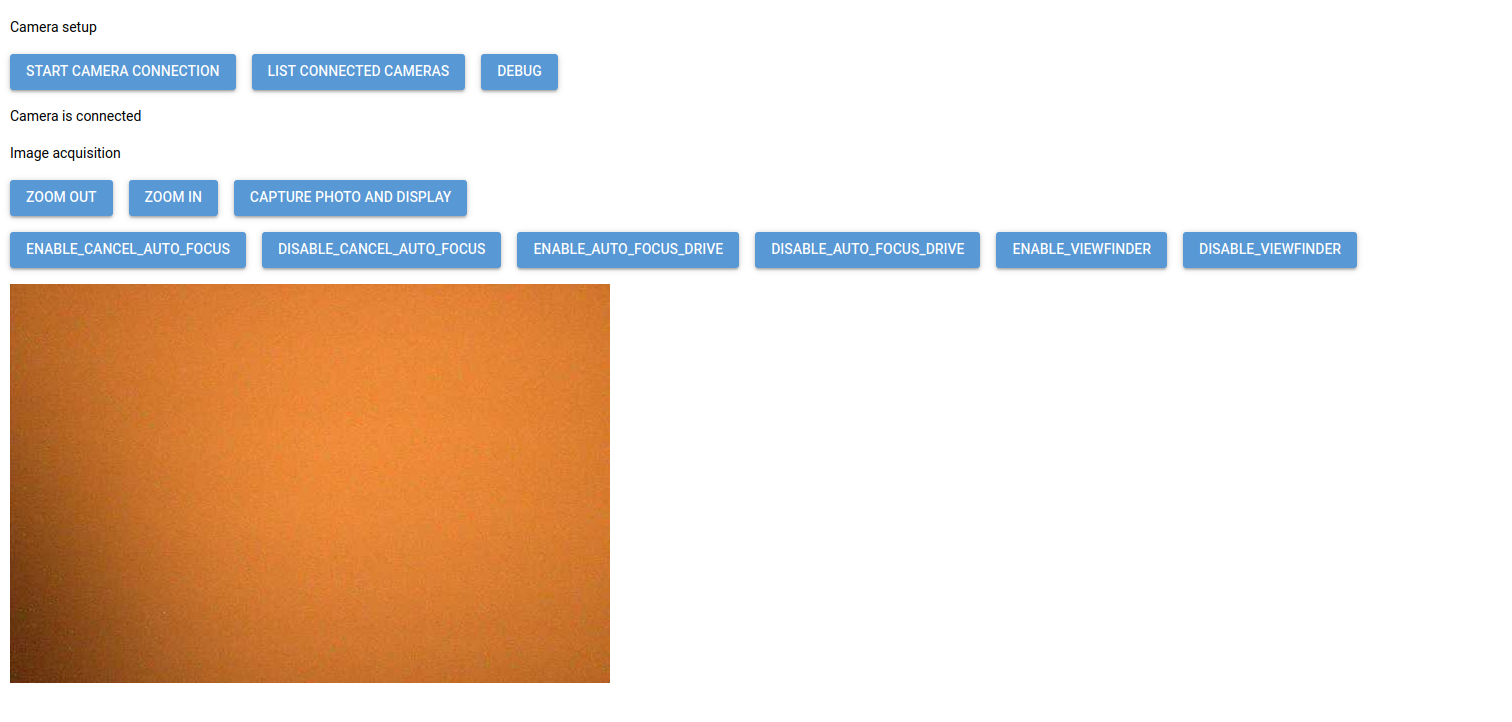
\includegraphics[width=1\textwidth]{Images/ui1.png}
\caption{Main screen with camera connection and photo capture features.}
\label{fig:ui_main_screen}
\end{figure}

\begin{figure}[h]
\centering
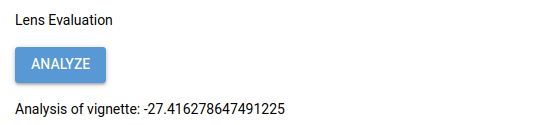
\includegraphics[width=0.8\textwidth]{Images/ui2.png}
\caption{Sketch of the screen with Analyze button and result of vignette analysis.}
\label{fig:ui_analysis_screen}
\end{figure}

\subsection{User Workflow}
Users can navigate through different scenarios for lens testing, including vignetting analysis using a white wall, PSF and bokeh analysis using point light sources, and sharpness analysis using test charts. The interface guides users through each scenario with clear instructions and feedback.

\section{Quality Assurance}

\subsection{Verification Methods}
[To be completed - how functionality is verified]

\subsection{Validation Procedures}
[To be completed - how results are validated]

\subsection{Performance Metrics}
[To be completed - what metrics are tracked]
